\chapter{Peer Network Activity Management}
\label{chap:pam}

Il sistema \textbf{\ac{PAM}} è stato il primo progetto in cui sono state
adottate le \ac{PBC}, segnando una svolta importante nel modo di sviluppare le applicazioni in \textit{Peer Network}.
In precedenza, l’infrastruttura della piattaforma di integrazione \ac{ESI}, che accoglie al suo interno
le \ac{PBC}, seguiva un’architettura monolitica. Tuttavia, l’implementazione di \ac{PAM} ha offerto un contesto
ideale per sperimentare e testare questa nuova metodologia. Il successo ottenuto
durante questa fase sperimentale ha dimostrato l’efficacia delle \ac{PBC}, non solo nel migliorare la
flessibilità e modularità del sistema, ma anche nel semplificare i processi di sviluppo. Questo ha
portato alla decisione strategica di estendere l’approccio basato sulle \ac{PBC} a tutte le
\ac{SBS} progettate successivamente per i clienti, segnando un’evoluzione
significativa nell’architettura delle applicazioni aziendali.

In questo capitolo vengono approfonditi i concetti introdotti precedentemente, riguardanti
le applicazioni componibili e le \ac{PBC}. Verrà esaminato come \textit{Peer Network} abbia
adottato e adattato questi principi nello sviluppo delle proprie \ac{SBS}, analizzandone la struttura
generale e il funzionamento. Successivamente, l’attenzione sarà focalizzata su \ac{PAM}, che rappresenta un
caso specifico di \ac{SBS}. Poiché \ac{PAM} e le \ac{SBS} condividono la stessa architettura strutturale basata sulle
\ac{PBC}, il sistema sarà utilizzato come esempio pratico per illustrare l’applicazione concreta di tali
concetti.

\section{Struttura di una Smart Business Solution}
\textit{Peer Network} utilizza Figura \ref{fig:sbs} e Figura \ref{fig:sbs-sap} per mostrare l'organizzazione delle
applicazioni componibili che sviluppa,
chiamate \ac{SBS} e progettate per diversi clienti e settori. Ciascuna
soluzione è composta da:
\begin{itemize}
    \item componenti backend, che integrano servizi e dati distribuiti su più piattaforme. Questa parte
    comprende inoltre la piattaforma di integrazione \ac{ESI}, responsabile della gestione delle \ac{PBC}
    necessarie;
    \item componenti frontend, sviluppati e successivamente distribuiti tramite la piattaforma Liferay\footnote{\url{https://www.liferay.com/it/home}}.
\end{itemize}

\begin{figure}
    \centering
    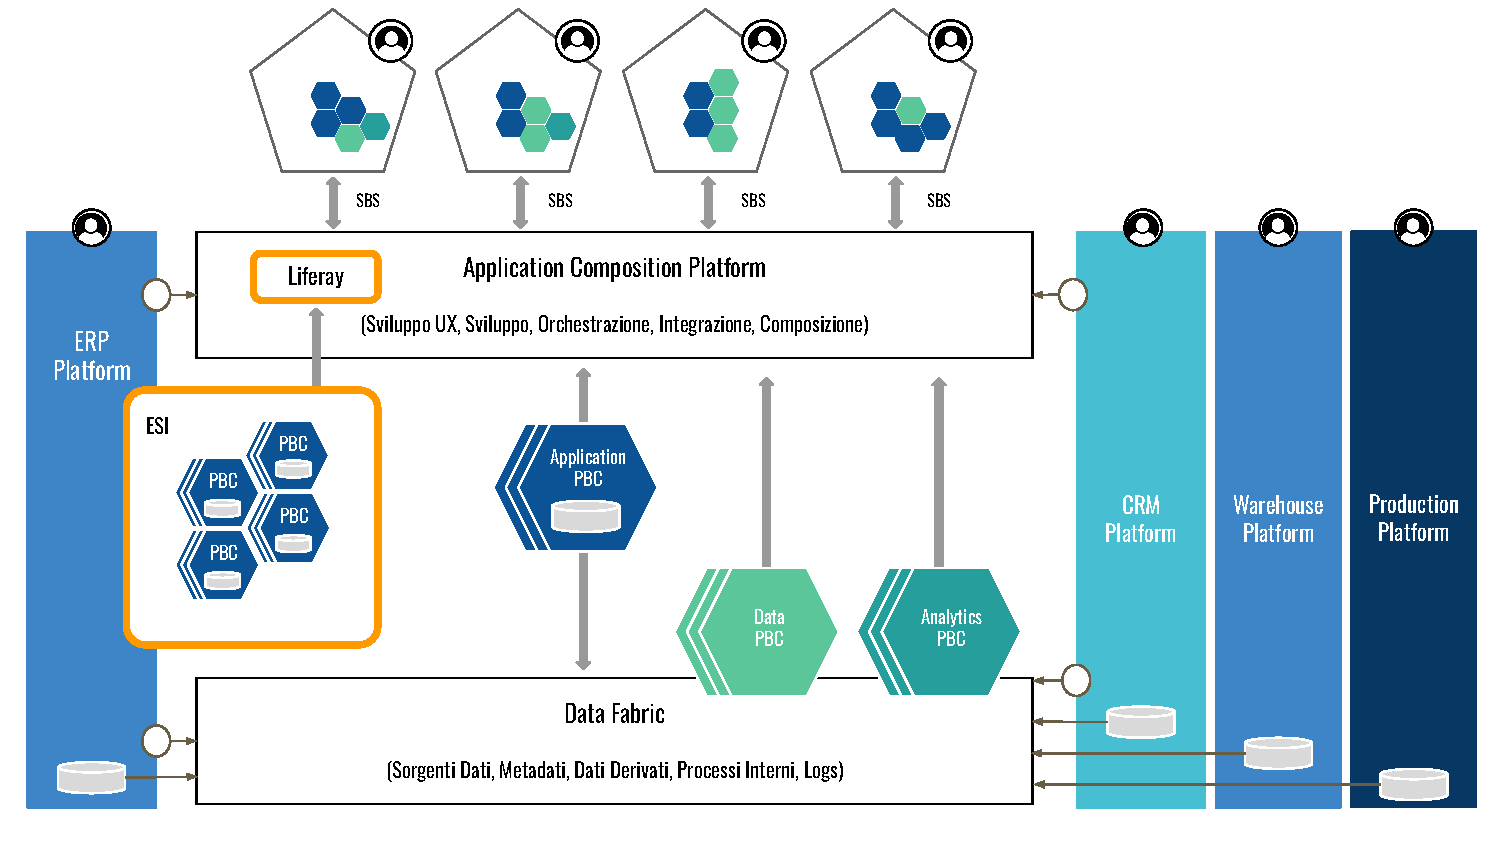
\includegraphics[width=\linewidth]{figures/struttura-sbs.pdf}
    \caption{Struttura di una \ac{SBS} e interazione tra i vari sistemi integrati}
    \label{fig:sbs}
\end{figure}

Dal punto di vista tecnico, ogni \ac{SBS} è composta da:
\begin{itemize}
    \item una parte di \textbf{backend}, che gestisce le logiche applicative ed è suddivisa in:
        \begin{itemize}
            \item \textbf{livello Data Fabric}, include sistemi informativi aziendali o database con cui la
            \ac{SBS} interagisce: ad esempio, può trattarsi di un \ac{ERP} (es. SAP), di un sistema \ac{CRM}
            (es. Salesforce) o di un database relazionale (es. MySQL). Poiché la maggior parte
            dei clienti utilizza sistemi SAP, le soluzioni si distinguono principalmente in SAP e non-SAP. In Figura
            \ref{fig:sbs-sap}, questo livello è rappresentato nella versione SAP;
            \item \textbf{livello \ac{PBC} Repository}, piattaforma \textbf{\ac{ESI}}: composto da \ac{PBC}, che forniscono accesso
            ai relativi dati e logiche applicative presenti nel livello Data Fabric. Le \ac{PBC}, pubblicate
            dalla piattaforma \ac{ESI}, fungono da intermediari tra le applicazioni e i sistemi informativi aziendali.
            A differenza di quanto formalizzato da Gartner, che individuava tre
            elementi base di una \ac{PBC}, dato, logiche e UI (opzionale), le \ac{PBC} di \textit{Peer Network} non contengono
            le rispettive interfacce utente, garantendo indipendenza tecnologica dal frontend. Sono state
            considerate due tipologie di \ac{PBC}:
            \begin{itemize}
                \item core: coprono funzionalità comuni a qualsiasi applicazione e cliente, quindi
                sono presenti in ogni \ac{SBS}. Nella Figura \ref{fig:sbs-sap} sono rappresentate dai cubi blu
                del livello PBC Repository;
                \item custom: realizzate per esigenze specifiche e applicazioni dedicate. Nella Figura \ref{fig:sbs-sap} sono rappresentate dai cubi
                arancioni del livello PBC Repository.
            \end{itemize}
            Le \ac{PBC} sono implementate come microservizi scritti in Kotlin\footnote{\url{https://kotlinlang.org}} e distribuite come container
            Docker\footnote{\url{https://www.docker.com}}, ciascuno contenente un gruppo coerente di \ac{PBC}. Ad esempio, G02 MATERIALS è il gruppo con
            funzionalità relative ai materiali, come il tipo di materiale PBC 0208 MATTYPE, la lista dei
            prezzi dei materiali PBC 0217 MATPRICELIST e l’unità di misura dei materiali PBC 0222 UNITOFMEASURE.
            In uno scenario on-premise (installazione presso il data-center del cliente), i
            microservizi sono orchestrati tramite Docker Compose. In uno scenario on-cloud, i
            microservizi vengono gestiti tramite Kubernetes\footnote{\url{https://kubernetes.io}}.
        \end{itemize}
    \item una parte di \textbf{frontend} chiamata \textbf{Composable layer}: è dedicata all’esperienza utente, il quale interagisce con
    la soluzione attraverso un'applicazione web.
    Anche il frontend viene realizzato come un insieme di moduli componibili (chiamati portlet)
    scritti in JavaScript utilizzando il framework Vue.js. Le portlet vengono assemblate in pagine web
    pubblicate tramite Liferay, seguendo un approccio componibile. Anche il frontend è gestito come
    microservizi, installati e orchestrati con modalità analoghe al livello \ac{PBC} Repository, sia in
    ambienti on-premise che cloud.
\end{itemize}

\begin{figure}
    \centering
    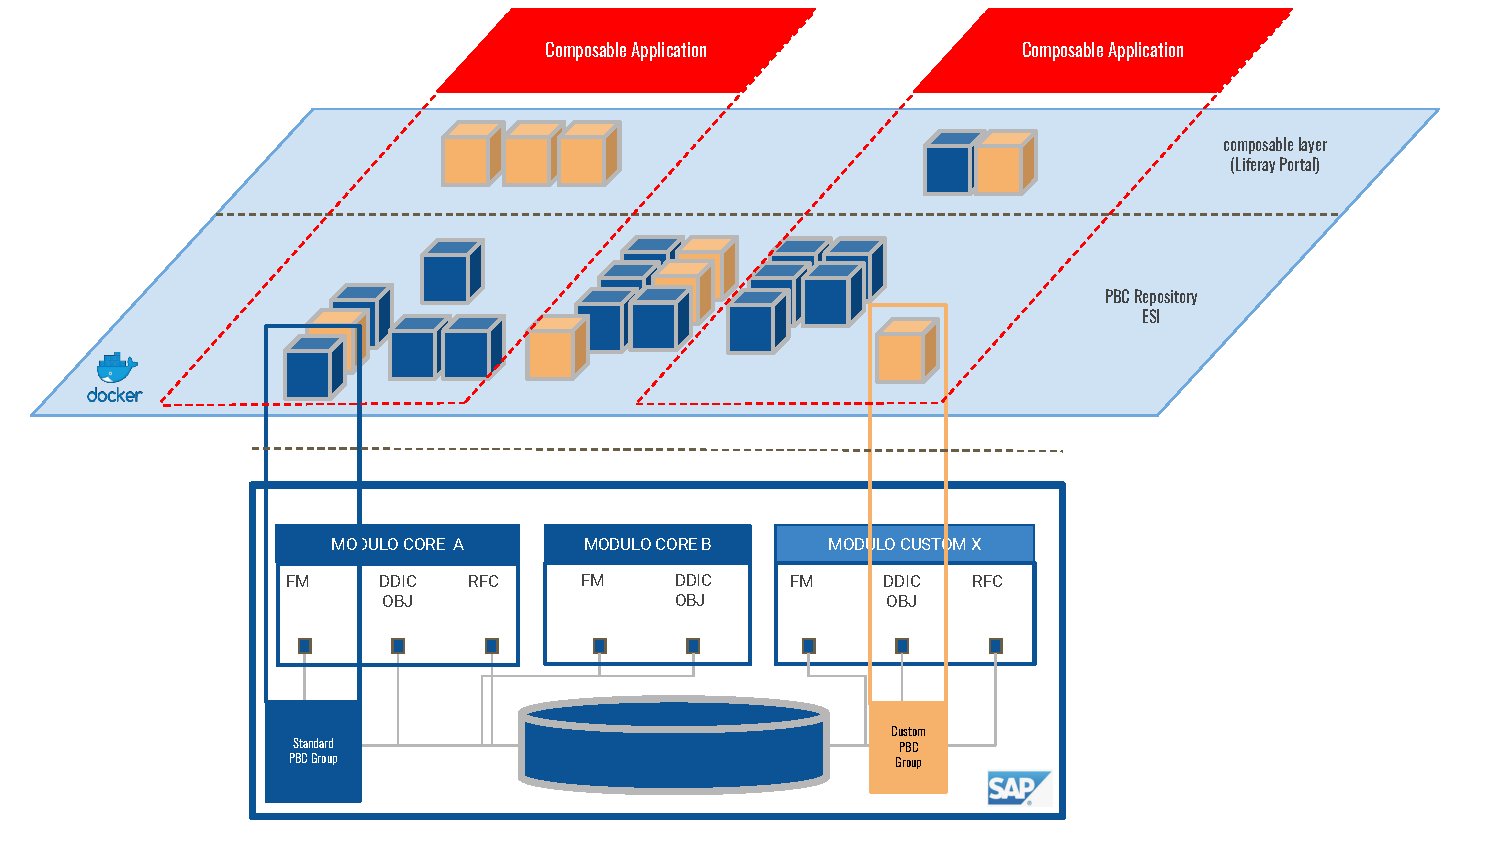
\includegraphics[width=\linewidth]{figures/architetturaSBS_SAP.pdf}
    \caption{Struttura di una \ac{SBS} che interagisce con un \ac{ERP} di SAP}
    \label{fig:sbs-sap}
\end{figure}

Entrando più nello specifico del livello \ac{PBC} Repository, la piattaforma \ac{ESI} gestisce le \ac{PBC}
attraverso due diversi livelli:
\begin{itemize}
    \item \textbf{livello API REST}: ospita i servizi di alto livello, cioè quelli riportati nella descrizione
    della \ac{PBC}. Questo strato è indipendente dallo scenario di implementazione ed è legato alla
    definizione dell’oggetto, così come la struttura dati;
    \item \textbf{livello sub-service}: ospita i servizi che interagiscono direttamente con lo strato dati
    della \ac{PBC}. I servizi implementati in questo livello differiscono a seconda del sistema informativo
    o database aziendale con il quale interagiscono:
    \begin{itemize}
        \item scenario SAP: i due layer API REST e sub-service sono gestiti da \ac{ESI} per SAP.
        In questo scenario il sub-service layer è costituito da BAPI, RFC e FM, oltre a servizi REST
        che interagiscono con la base dati dell'\ac{ERP} di SAP;
        \item scenario non-SAP: i due layer API REST e sub-service sono gestiti dalla versione
        di \ac{ESI} non-SAP. In questo scenario il sub-service layer è costituito da servizi che
        interagiscono con un database relazionale.
    \end{itemize}
\end{itemize}

    \subsection{Struttura di Peer Network Activity Management}
    Considerando l’architettura delle \ac{SBS} descritta in precedenza, quella di \ac{PAM} include:
    \begin{itemize}
        \item un modulo di backend che comprende:
        \begin{itemize}
            \item la base dati: come piattaforma per il database viene usato MySQL ed è installato presso il
            cloud provider OVH\footnote{\url{https://www.ovhcloud.com}} su una macchina proprietaria;
            \item le logiche che interagiscono con la base dati e i servizi relativi, viene usato
            \ac{ESI} non-SAP (installato presso il cloud provider OVH su una macchina proprietaria) come
            strumento di esposizione dei servizi e integrazione con le componenti di frontend.
        \end{itemize}
        \item un modulo di frontend che gestisce la UX/UI dell’applicazione, realizzato su
        Liferay Community Edition installato presso il cloud provider OVH su una macchina proprietaria.
    \end{itemize}

\section{Attività svolte}
Le attività di sviluppo hanno riguardato l’applicazione \ac{PAM}, un software utilizzato internamente all’azienda
per la gestione di aspetti organizzativi e burocratici. Il lavoro si è concentrato principalmente sullo
sviluppo frontend, utilizzando anche alcuni servizi esposti dalle \ac{PBC}, oltre ad un breve intervento
dedicato alla modifica di alcuni dati all'interno del database relazionale.

    \subsection{Sviluppo nell'area Progetti}
    \begin{figure}
        \centering
        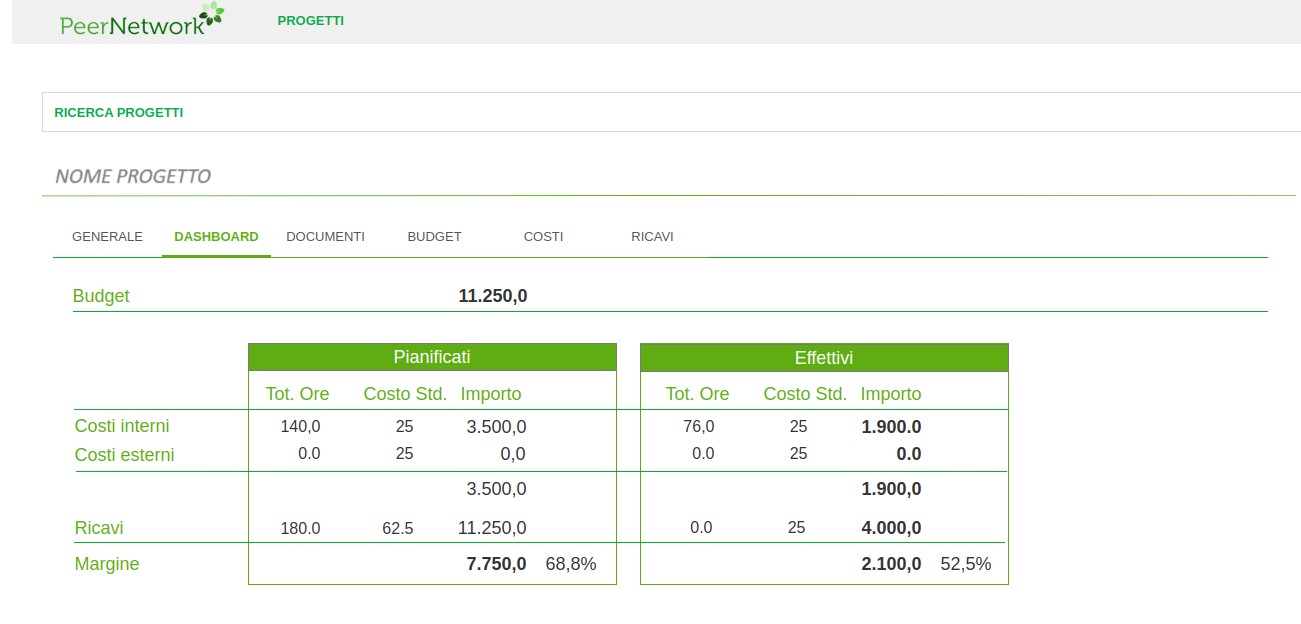
\includegraphics[width=\linewidth]{figures/pam-dashboard.png}
        \caption{Mockup esplicativo della dashboard richiesta}
        \label{fig:mockup-pam}
    \end{figure}

    Nell’area Progetti dell’applicativo \ac{PAM} sono raccolte tutte le informazioni relative
    ai progetti sviluppati. Per ciascuno di essi è disponibile un riepilogo dettagliato che include gli aspetti
    organizzativi, come la composizione del team, le tariffe orarie in base al ruolo, il budget assegnato
    e altri dati economici.

    Osservando il mockup in Figura \ref{fig:mockup-pam}, si nota che la sezione dedicata allo stato economico
    del progetto comprende costi, ricavi e margini, sia pianificati che reali. I valori previsionali
    vengono definiti all’inizio del progetto sulla base del budget disponibile concordato
    con il cliente, inserito nel sistema dal project manager. I dati effettivi, invece, si aggiornano in modo automatico.
    I tempi di lavoro vengono registrati dai dipendenti su Jira e poi sincronizzati in \ac{PAM} attraverso i \textbf{timeLog}.
    Un timeLog rappresenta una sessione di lavoro svolta da un utente su una specifica attività di un determinato progetto ed è caratterizzato da
    data, durata e descrizione dell’attività svolta. Oltre ai dati sui tempi di lavoro, il sistema integra anche le
    informazioni relative alle pre-fatture, che vengono generate dai project manager e dall’amministrazione all’inizio
    della fase di fatturazione.
    
    Per il recupero dei dati previsionali, viene utilizzata l’azione \texttt{projectGetDetails}, fornita dalla PBC 0801 PROJECT
    all’interno del GROUP G08 PROJECTS. Il budget di progetto rappresenta il valore economico totale assegnato ed è
    il punto di partenza per la definizione degli altri valori.

    In particolare, i \textbf{dati pianificati} vengono calcolati sulla base delle informazioni iniziali del progetto:
    \begin{itemize}
        \item costi interni: il totale delle ore viene determinato trasformando il numero di giornate a budget in ore e
        moltiplicando il risultato per un costo standard del dipendente;
        \item costi esterni: costi derivanti dall’impiego di risorse esterne, come le aziende partner. L’importo è dato
        dalla tariffa giornaliera concordata con il partner per il numero delle giornate assegnate alla risorsa;
        \item ricavi: l’importo corrisponde al budget assegnato al progetto, mentre il costo orario standard viene
        determinato in base al ruolo dei dipendenti coinvolti. La tariffa giornaliera dei dipendenti viene recuperata
        tramite l’azione \texttt{projectRateGetList} della PBC 0807 PROJECT RATE, appartenente al GROUP G08 PROJECTS. Il totale
        delle ore viene quindi calcolato dividendo il budget assegnato per la tariffa;
        \item margine: si ottiene come differenza tra l’importo dei ricavi e quello dei costi. La percentuale di margine
        viene calcolata rapportando questo valore rispetto ai ricavi complessivi.
    \end{itemize}

    I \textbf{dati effettivi}, invece, vengono aggiornati in tempo reale sulla base delle informazioni registrate nel sistema
    durante l’avanzamento del progetto:
    \begin{itemize}
        \item costi interni: il totale delle ore è dato dalla somma di tutte quelle effettivamente caricate dai
        dipendenti su Jira. Il recupero di questi dati avviene tramite l’azione timeLogGetList dalla PBC 0803 TIMELOG
        nel GROUP G08 PROJECTS, mentre costo standard e importo vengono ricalcolati secondo la stessa logica dei dati pianificati;
        \item costi esterni: costi derivanti dall’impiego di risorse esterne, come per i dati pianificati;
        \item ricavi: il valore è dato dalla somma di tutte le pre-fatture emesse per il progetto, estratte con l’azione
        \texttt{preInvoiceGetList}. Poiché la pre-fattura
        è un concetto specifico dell’applicativo \ac{PAM}, è stata adattata la PBC INVOICE del GROUP G16 1601 INVOICING,
        facendola diventare PAM PREINVOICE;
        \item margine: sia l’importo che la percentuale vengono calcolati secondo la stessa metodologia utilizzata per i dati pianificati.
    \end{itemize}

    \subsection{Aggiornamento database}
    Durante l'implementazione della dashboard riepilogativa dei dati economici di un progetto, è emerso un
    disallineamento nei totali delle pre-fatture visualizzate. Il problema è stato individuato confrontando
    i dati mostrati nella dashboard con quelli disponibili nell'area del portale denominata Attività Mensili,
    in particolare nella sezione che permette di visualizzare l’elenco completo delle pre-fatture associate a un cliente.
    Un'analisi approfondita ha evidenziato che l'incongruenza era dovuta a un disallineamento dei dati nel
    database. Nello specifico, per le prime pre-fatture generate tramite il portale a novembre 2024, il sistema
    non prevedeva ancora il salvataggio del progetto di riferimento, funzionalità introdotta solo nei mesi successivi.
    Per risolvere il problema, è stato necessario aggiornare i record incompleti direttamente in produzione tramite
    uno script MySQL. Lo script ha incrociato i dati di diverse tabelle del database per risalire ai valori corretti
    e garantire l'allineamento delle informazioni.

    \subsection{Modifiche nell'area Attività Mensili}
    Sono state apportate alcune modifiche per rendere l'area Attività Mensili più intuitiva ed efficiente.
    Questa sezione, già in uso, permette di monitorare e rendicontare mensilmente le ore di lavoro dei dipendenti
    sui vari progetti, oltre a generare automaticamente i report mensili da allegare alle fatture destinate ai
    clienti. Le principali modifiche grafiche introdotte sono state:
    \begin{itemize}
        \item l'inserimento di un form con input e pulsante di salvataggio: è stata aggiunta la possibilità di
        modificare alcuni campi della testata delle pre-fatture, come il numero AGO e il numero CRM, sia nella
        sezione Pre-fatture che in quella di Controllo Amministrazione. A tal fine, è stato introdotto un pulsante
        di salvataggio accanto a ogni pre-fattura modificabile;
        \item l'aggiunta di righe verticali per separare i campi: nella sezione riepilogativa delle Pre-fatture
        è stata implementata una riga divisoria tra le colonne dello specchietto riassuntivo, dove vengono
        visualizzati i totali del fatturato se le pre-fatture sono standard o manuali. Poiché il numero di
        colonne può variare dinamicamente, la riga viene mostrata solo se sono presenti almeno due colonne di valori;
        \item l'allineamento dei campi e riduzione dello spazio bianco: per migliorare la leggibilità dell’interfaccia,
        è stata ridotta la distanza tra i dati di testata della Pre-fattura, sia nella sezione Pre-fatture che in quella
        di Controllo Amministrazione.
    \end{itemize}

    Oltre ai cambiamenti grafici, sono state sviluppate logiche per garantire la correttezza di alcuni dati
    visualizzati e gestiti dall’applicativo, come:
    \begin{itemize}
        \item il salvataggio dei valori inseriti nel form: è stato implementato il meccanismo per permettere il salvataggio
        nel database dei valori AGO e CRM delle pre-fatture modificati dagli utenti. In questo modo, le informazioni
        aggiornate vengono conservate correttamente e rese disponibili per le successive elaborazioni;
        \item la correzione del calcolo dell’importo totale delle pre-fatture: nella sezione Controllo Amministrazione, è
        stato verificato e corretto il calcolo del totale da fatturare. Il problema risiedeva nel fatto che il sistema
        non considerava le pre-fatture manuali, ovvero quelle create dall’amministrazione ma che non
        derivano dal flusso standard di conferma delle ore in Jira. Ora il riepilogo tiene conto di entrambe le tipologie
        di pre-fatture, sia quelle standard che quelle manuali;
        \item l'assegnazione corretta del creatore di ogni pre-fattura: nelle sezioni Controllo Amministrazione e Pre-fatture,
        il campo relativo al project manager responsabile della pre-fattura non veniva correttamente visualizzato.
        Il problema è stato risolto implementando un meccanismo di recupero del project
        manager corretto per ogni pre-fattura, garantendo la corretta associazione dei dati.
    \end{itemize}